\documentclass[UTF8]{ctexart}
\usepackage{amsmath}
\usepackage{amsfonts}
\usepackage{amssymb}
\usepackage{graphicx}
\usepackage{hyperref}
\usepackage{float}
\usepackage{caption}
\usepackage{subfig}
\usepackage{bm}
\usepackage{mathrsfs}
\usepackage{latexsym}
\usepackage{euscript}
\usepackage{esint}
\usepackage{blindtext}
\usepackage{multirow}
\renewcommand\thesection{\Roman{section}}

\hypersetup{colorlinks=true,linkcolor=black}

% Title Page
\title{NaI(TI)闪烁谱仪实验报告}
\author{17377306\ 马晓天}
\RequirePackage[a4paper]{geometry}
\geometry{
	textwidth=138mm,
	textheight=215mm,
	left=27mm,
	right=27mm,
	top=25.4mm, 
	bottom=25.4mm,
	headheight=2.17cm,
	headsep=4mm,
	footskip=12mm,
	heightrounded,
}


\begin{document}
\maketitle

\thispagestyle{empty}
\section{数据分析}
实验条件为：$^{60}$Co放射源，$^{137}$Cs放射源，$ \rm LaBr_{3} $探测器(型号未记录)，高压电源为600V，放大器放大倍数为$ 0.5\times500=250 $($^{60}$Co贴近探测器时放大倍数为$ 0.5\times200=100 $)，道数为4096。
实验原始数据为:
\begin{table}[H]
	\centering
	\caption{ROI相关数据}
	\begin{tabular}{ccccccc}
		\hline
		ROI & centroid/ch & FWHM/ch & $ \eta $ & $ N_{\rm net} $ & $ t_{\rm r} $/s &$ t_{\rm l} $/s\\
		\hline
		\multirow{3}[0]{*}{$\rm ^{60}Co$} & 2320.09 & 49.31 & 0.02125 & 135688 &&\\
		 & 2636.03 & 53.34 & 0.02024 & 122954 &470&464\\
		 & 2892.38 & 76.08 & 0.02630 & 30953 &&\\
		\hline
		\multirow{2}[0]{*}{$\rm ^{137}Cs$} & 1304.85 & 37.35 & 0.02862 & 229947 &\multirow{2}[0]{*}{423}&\multirow{2}[0]{*}{418}\\
		 & 2888.86 & 80.61 & 0.02790 & 28428 &&\\
		\hline
		 & 1299.39 & 38.13 & 0.02934 & 275173 &&\\
		\multirow{2}[0]{*}{$\rm ^{60}Co$和$\rm  ^{137}Cs $} & 2312.36 & 49.00 & 0.02119 & 113581 &\multirow{2}[0]{*}{498}&\multirow{2}[0]{*}{489}\\
		 & 2626.84 & 51.19 & 0.01949 & 104213 &&\\
		& 2883.78 & 58.48 & 0.02028 & 20921 &&\\
		\hline
		本底 & 2886.69 & 71.13 & 0.02464 & 13037 & 183 &183\\
		\hline
		 & 875.48 & 24.18 & 0.02762 & 517630 &&\\
		$\rm ^{60}Co$贴近 & 998.37 & 24.96 & 0.02500 & 459438 &213&196\\
		 & 1902.31 & 29.74 & 0.01563 & 55232 &&\\
		\hline
	\end{tabular}
\end{table}
其中，ROI代表选的峰值区域，centroid是峰值对应道址，FWHM是半高宽，$ \eta $是能量分辨率，$ N_{\rm net} $是峰的净计数, $ t_{\rm r} $是实际测量时间，$ t_{\rm l} $是测量活时间。

\subsection{$\gamma$射线能谱测定}
图1、图2分别为$\rm ^{60}Co $和$\rm ^{137}Cs $的能谱,图1中：A为1.173MeV对应的$\gamma$射线全能峰，B为1.332Me
\begin{sloppypar}
	\parindent=0pt
V对应的$\gamma$射线全能峰，C为环境本底峰，D为反散射峰(能量约200keV)，E为康普顿平台，图2中：A为0.662MeV对应的$\gamma$射线全能峰，B为环境本底峰，C为反散射峰(能量约200keV)，D为康普顿平台。图3、图4为示波器中捕捉到的$ \gamma $全能峰，其中$\rm ^{60}Co $有2个全能峰在示波器中出现频率高，对应1.173MeV(从下向上第二个峰)和1.332MeV(从下向上第一个峰)的$ \gamma $射线，$\rm ^{137}Cs $有1个全能峰(从上向下第一个峰)在示波器中出现频率高，对应0.662MeV的$ \gamma $射线。
\end{sloppypar}
\begin{figure}[H]
	\begin{minipage}[t]{0.5\textwidth}
		\centering
		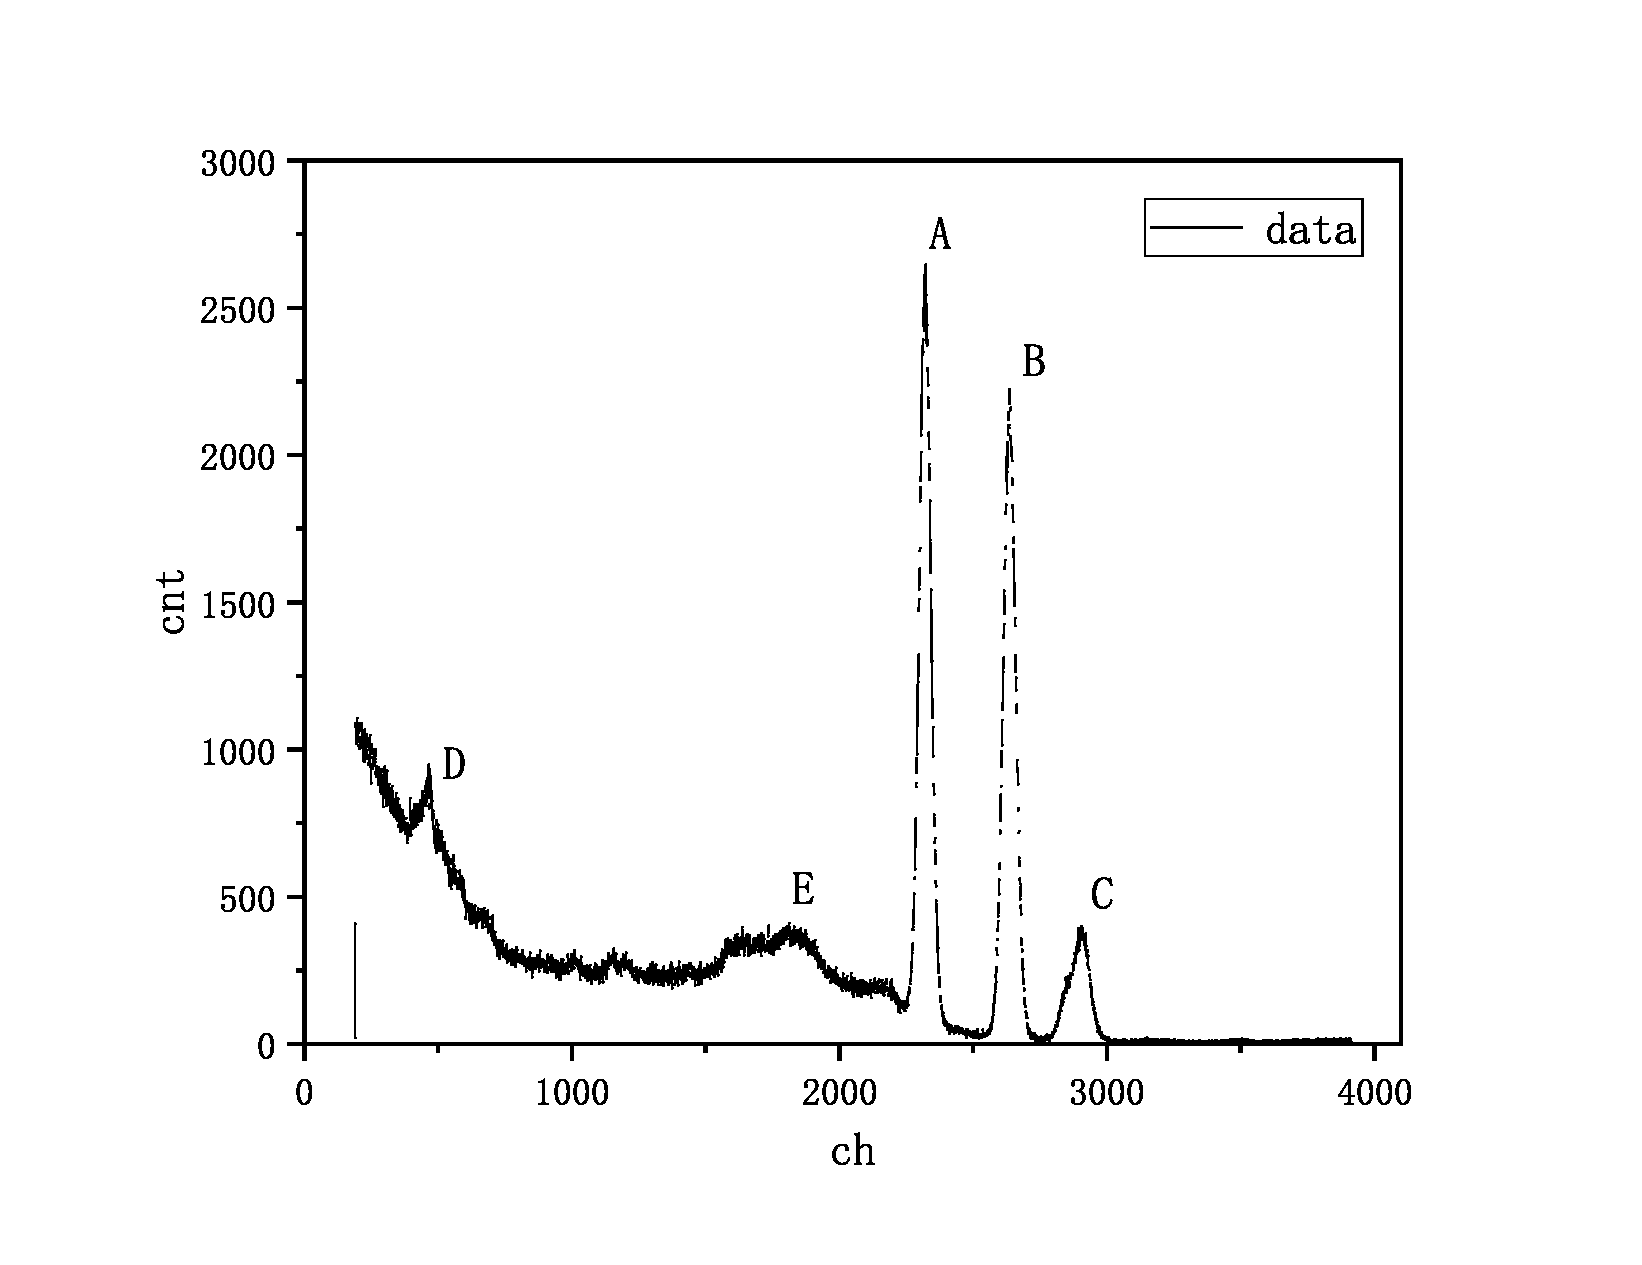
\includegraphics[width=1.1\linewidth]{Co60.eps}
		\caption{$\rm ^{60}Co $的$\rm cnt-ch $曲线}
	\end{minipage}
	 \
	\begin{minipage}[t]{0.5\textwidth}
		\centering
		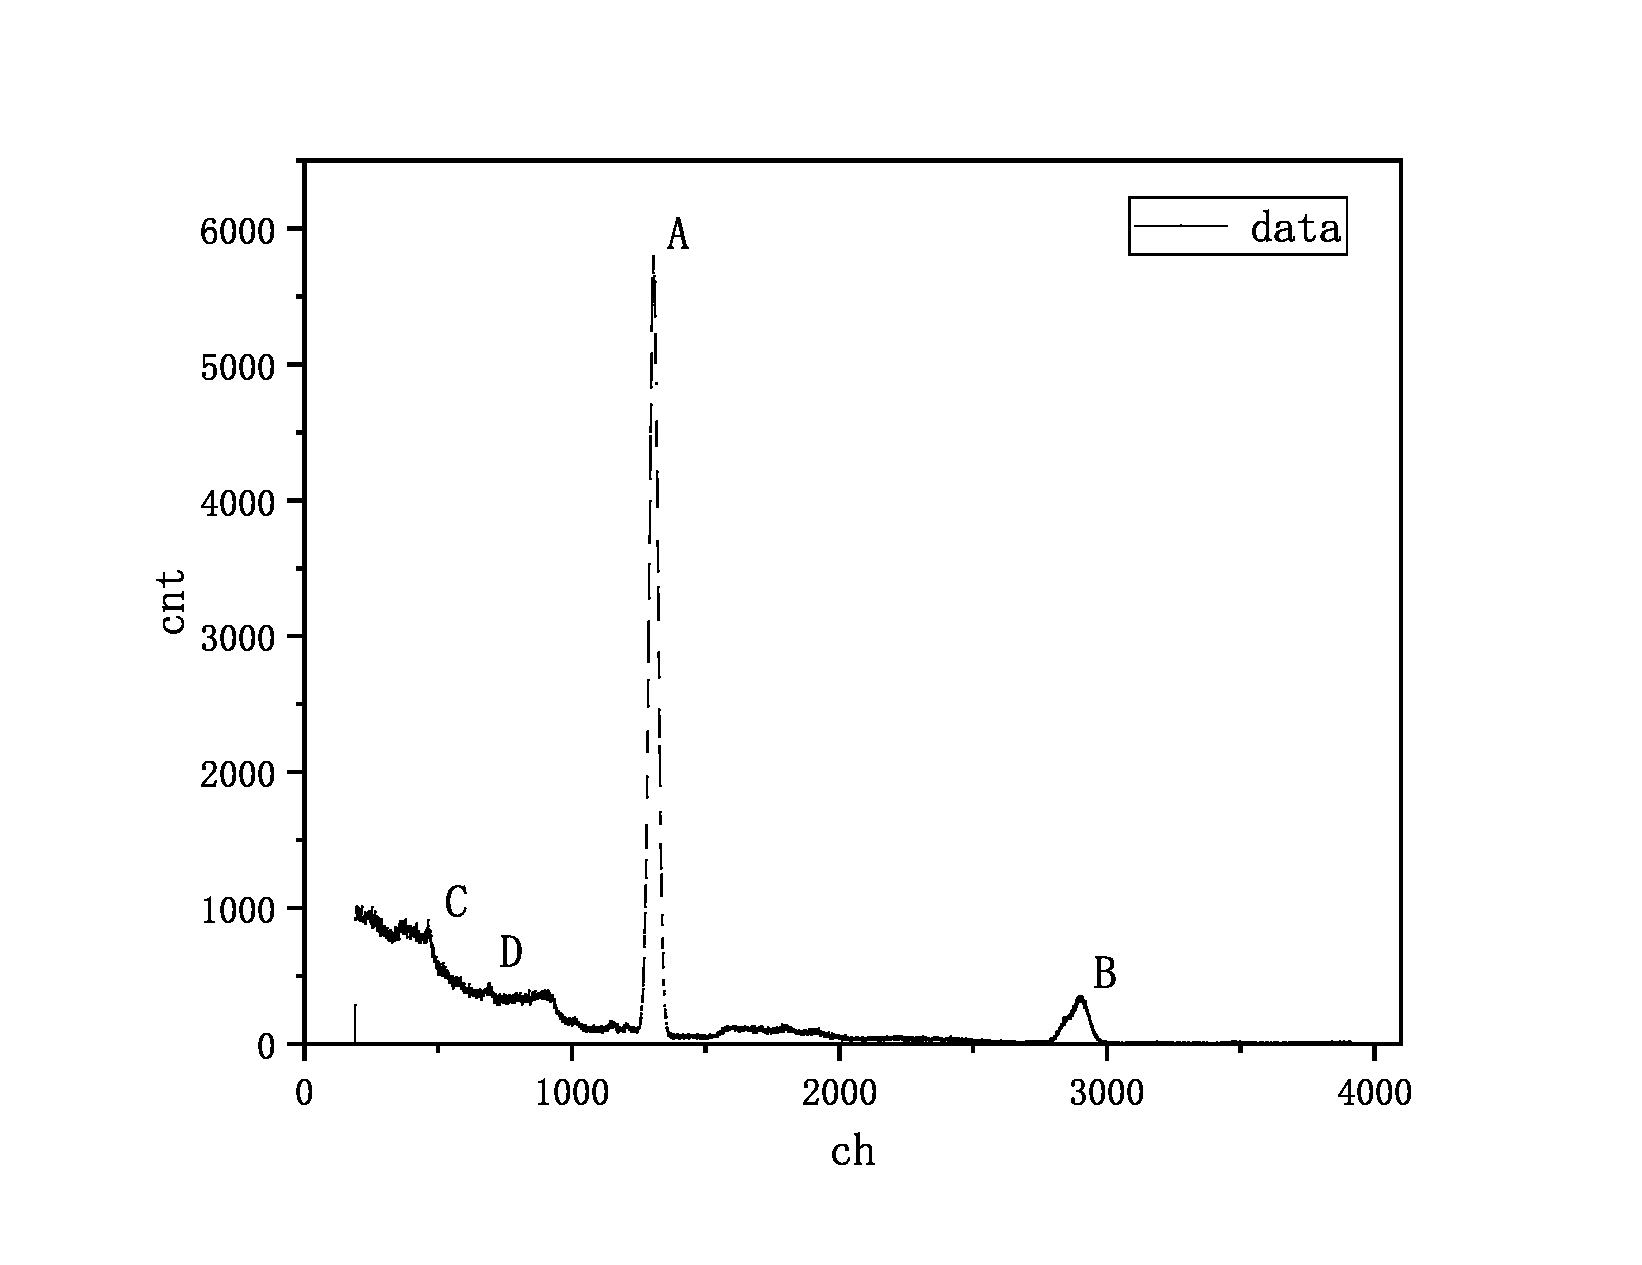
\includegraphics[width=1.1\linewidth]{Cs137.eps}
		\caption{$\rm ^{137}Cs $的$\rm cnt-ch $曲线}
	\end{minipage}
\end{figure}

\begin{figure}[H]
	\begin{minipage}[t]{0.5\textwidth}
		\centering
		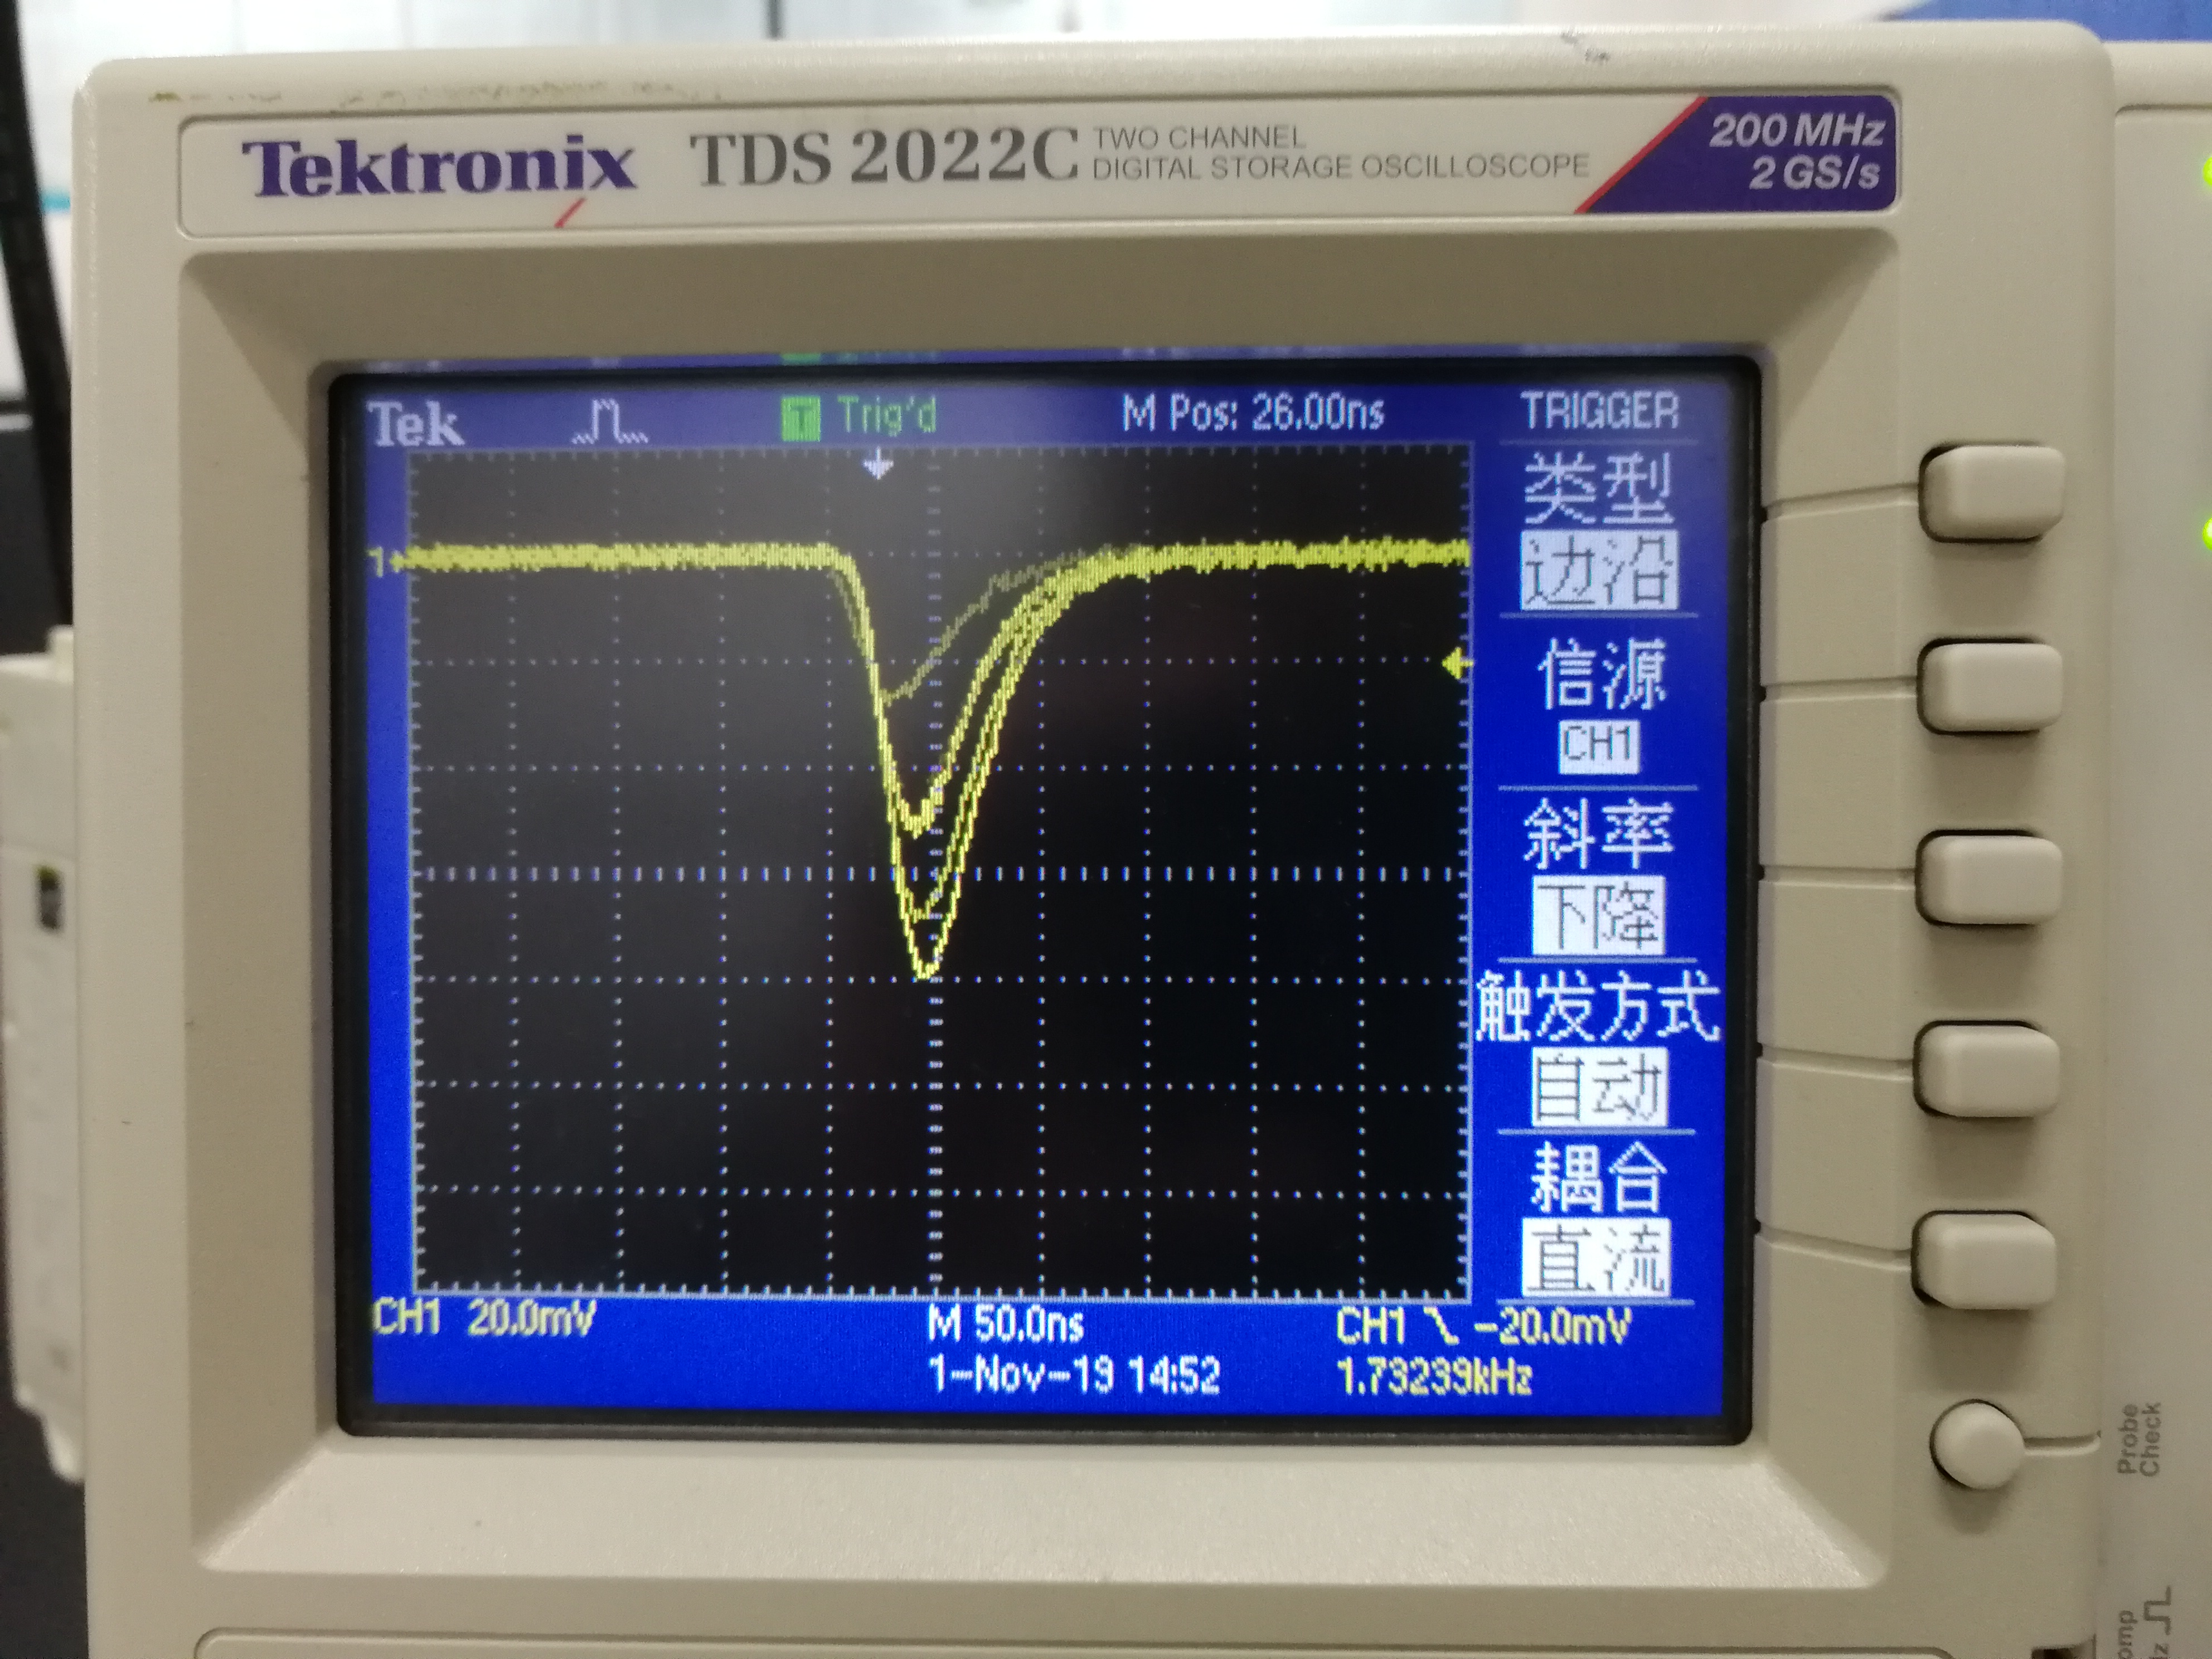
\includegraphics[width=0.9\linewidth]{Co60.jpg}
		\caption{$\rm ^{60}Co $的全能峰捕捉图}
	\end{minipage}
	\quad
	\begin{minipage}[t]{0.5\textwidth}
		\centering
		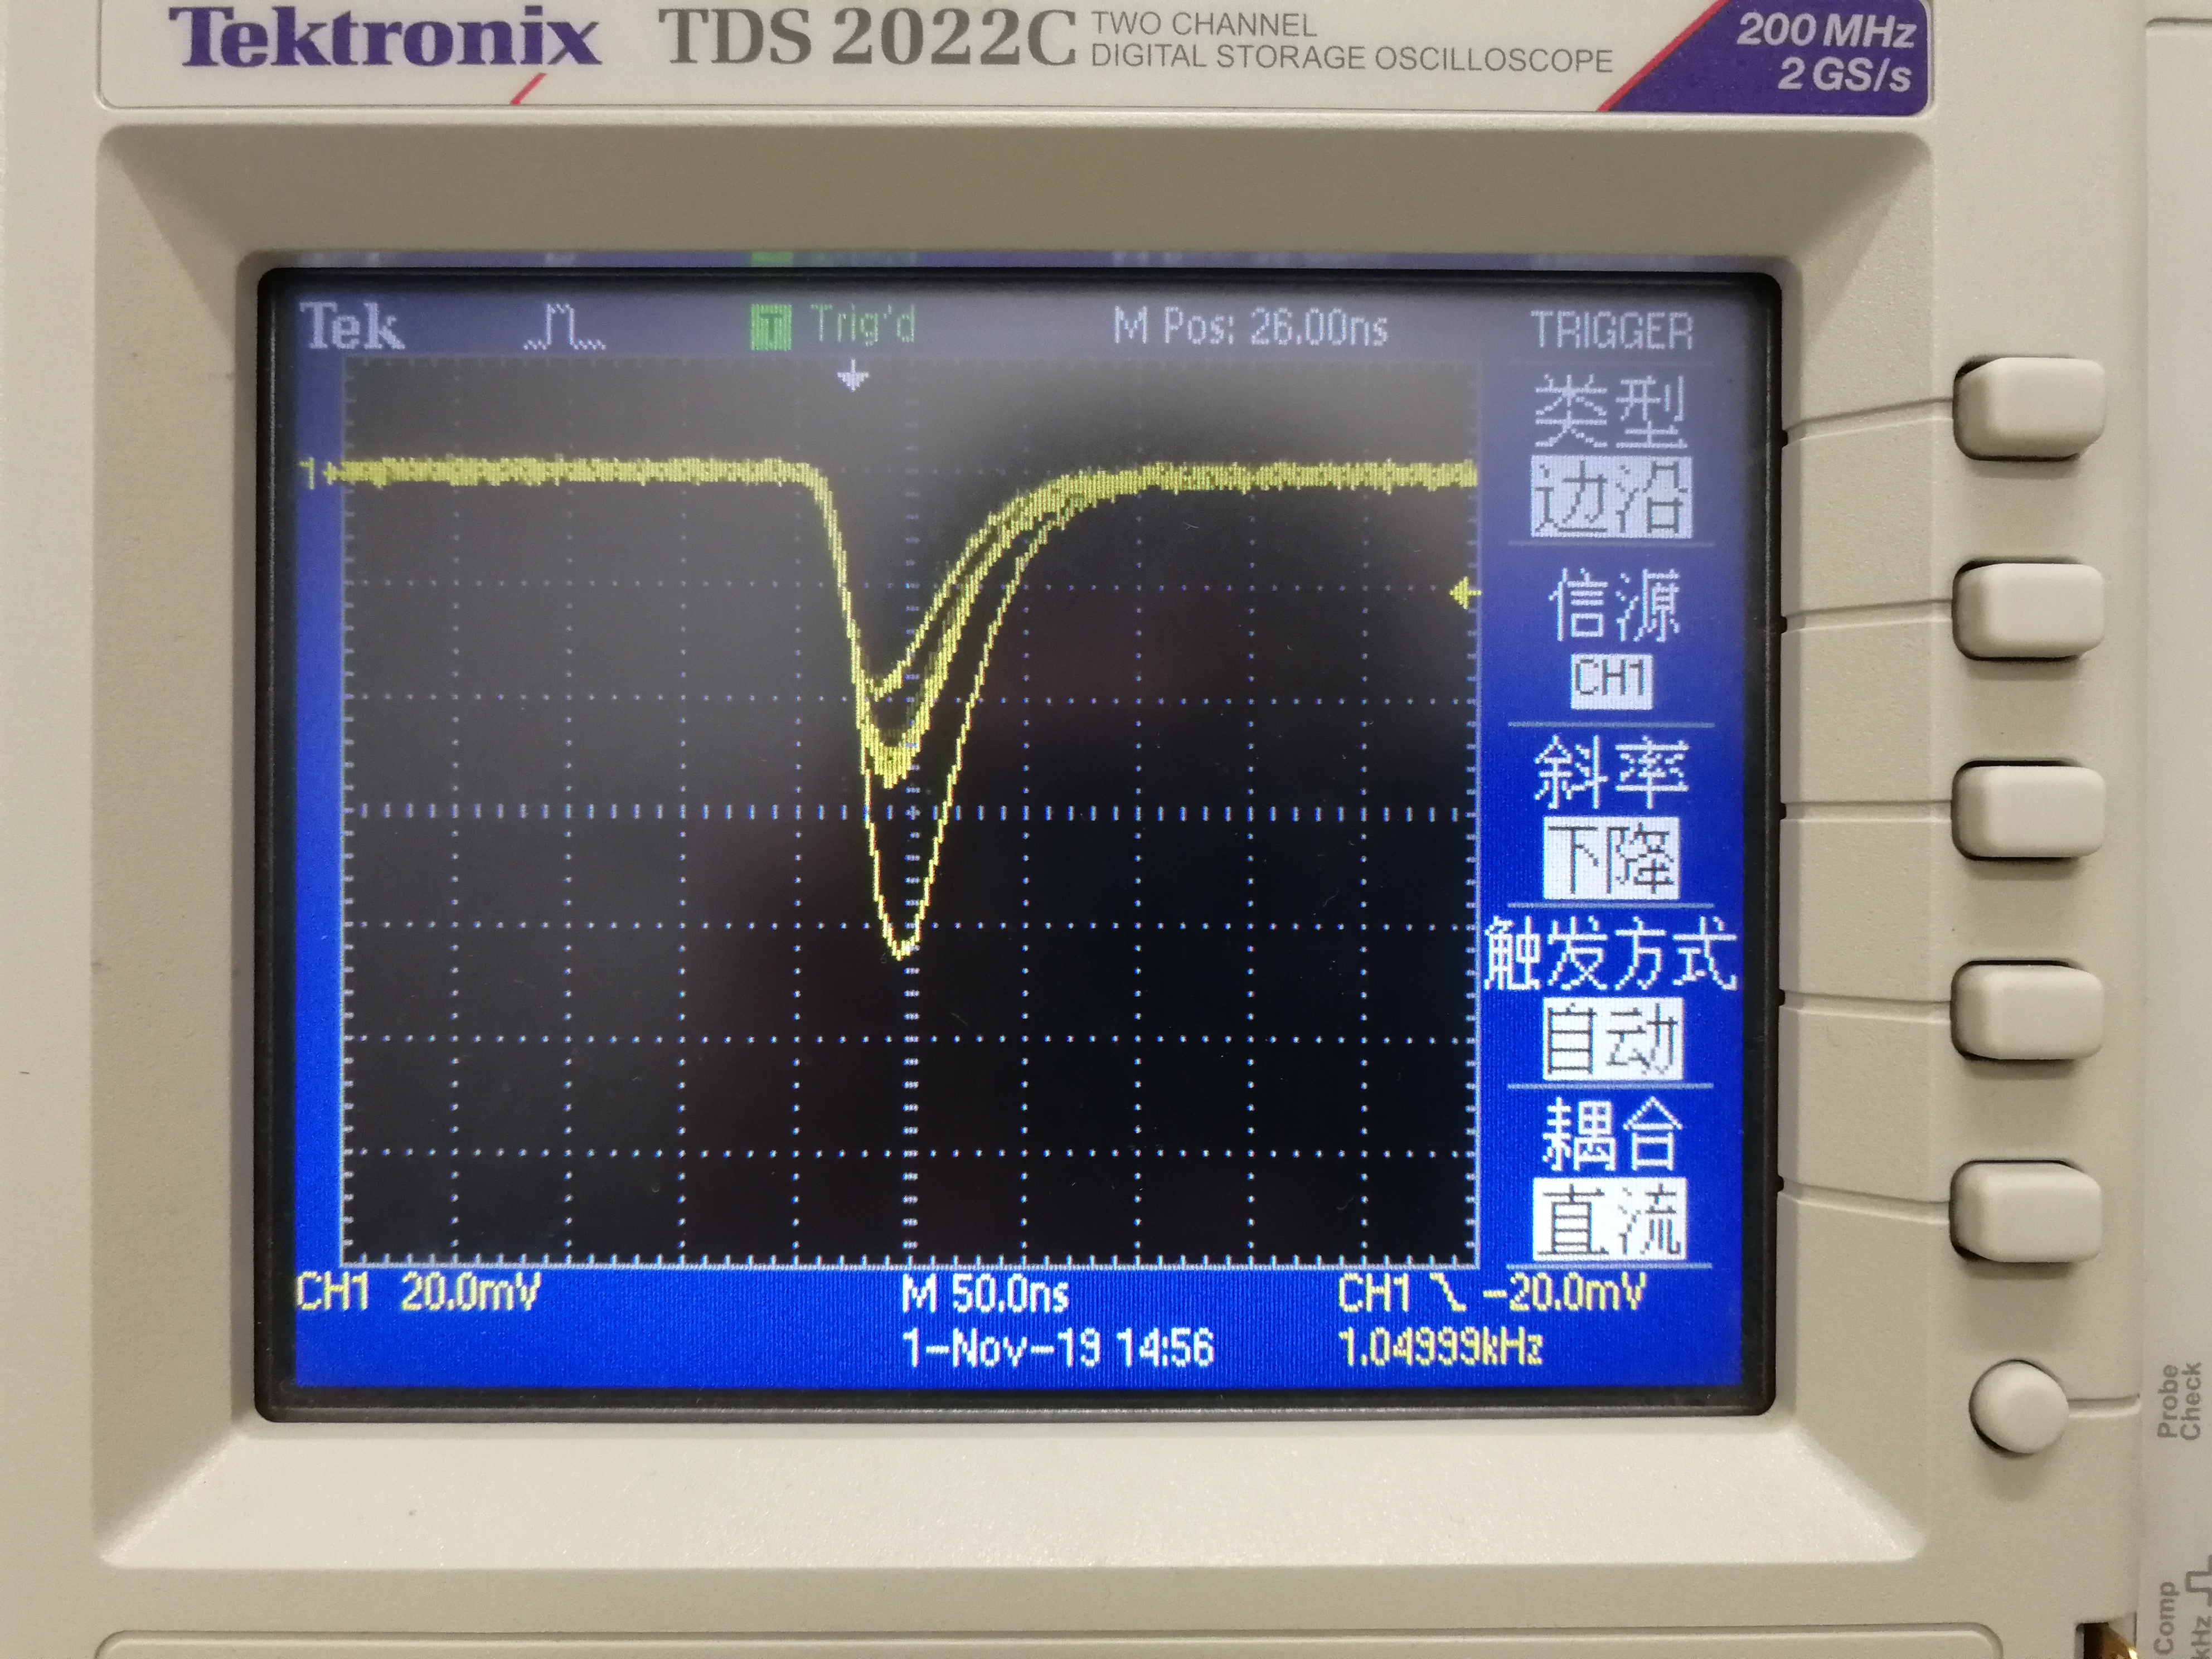
\includegraphics[width=0.9\linewidth]{Cs137.jpg}
		\caption{$\rm ^{137}Cs $的全能峰捕捉图}
	\end{minipage}
\end{figure}

\subsection{能量刻度}
能量$ E $与峰位(道址)$ x_{\rm p} $的关系式为：
\begin{equation}
E(x_{\mathrm{p}})=Gx_{\mathrm{p}}+E_{0}
\end{equation}
利用已知数据(0ch,0keV)，(1299ch,662keV)，(2627ch,1332keV)，采用如下函数族进行拟合：
\begin{equation}
y=a+bx
\end{equation}
拟合得到：
\begin{equation*}
a=1.049\pm2.316,b=0.507\pm0.001,R^2=0.99999
\end{equation*}
对比式(1)(2)得：
\begin{equation}
G=b=0.507\pm0.001
\end{equation}
\begin{equation}
E_0=a=1.049\pm2.316
\end{equation}
故关系式为：
\begin{equation}
E(x_{\mathrm{p}})=(0.507\pm0.001)x_{\mathrm{p}}+(1\pm2)(\rm keV)
\end{equation}
拟合曲线如图5，由此可推断出$\rm ^{60}Co $第二个峰($  x_{\rm p}=2312 $)对应能量为$ E=(1173\pm3)\rm keV $
\begin{figure}[H]
	\centering
	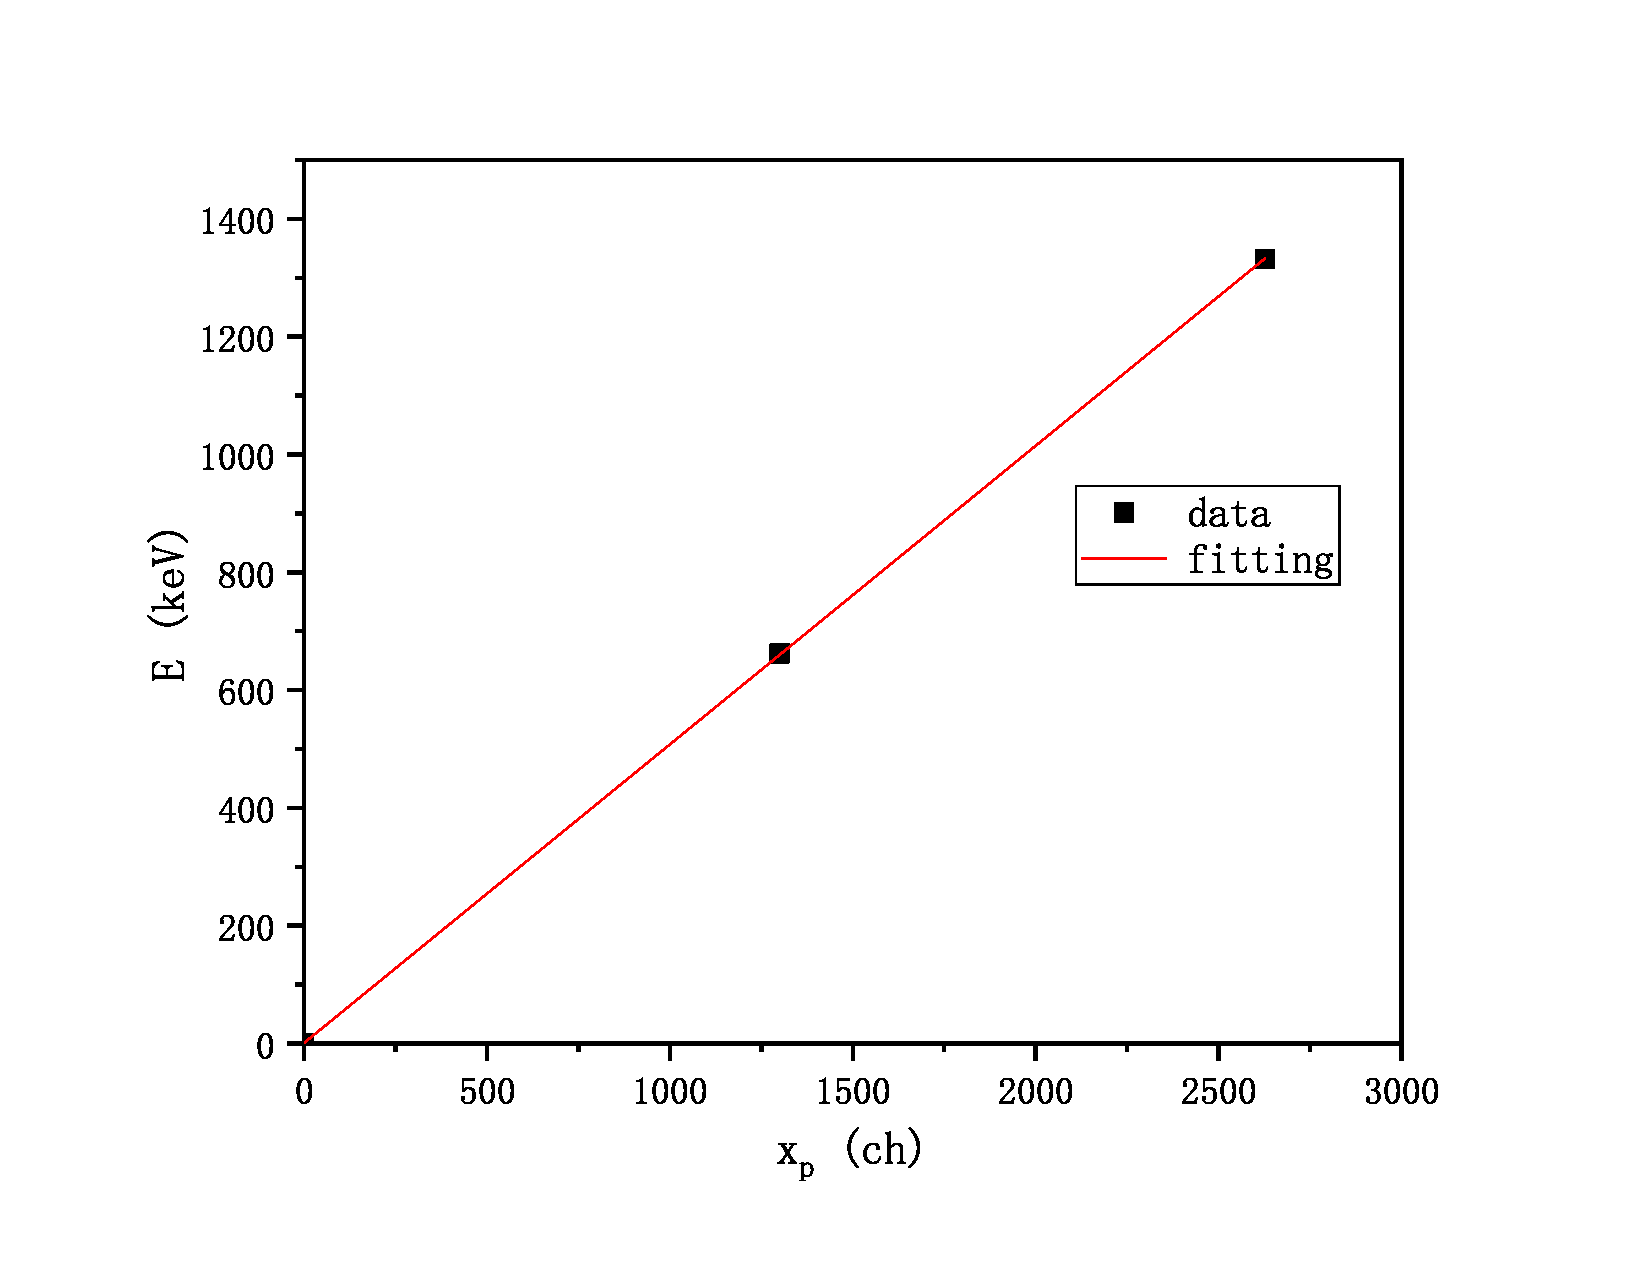
\includegraphics[width=0.9\linewidth]{E-xp.eps}
	\caption{$ E-x_{\rm p} $直线}
\end{figure}

\subsection{能量分辨率随射线能量的关系}
能量分辨率$ \eta $与能量$ E $以及多道道数(CH)的关系式为：
\begin{equation}
\eta=\frac{\Delta E}{E}=\frac{\Delta H}{H_{0}}=\frac{\Delta(\mathrm{CH})}{\mathrm{CH}}
\end{equation}
%\begin{sloppypar}
%	\parindent=0pt
 其中$\rm \Delta(CH) $为峰值(记数率极大值)一半处的宽度(或称半宽度)，记作FWHM，CH为记数率极大处的脉冲幅度。由于能量与道址为线性关系(在上面已拟合出线性关系式)，故可绘制能量分辨率$\eta$与峰位(道址)$ x_{\rm p}$的关系图，进而反映它与射线能量的关系，如图6。其中在2900道附近的能量分辨率变化过大，将其舍弃后发现剩余点的变化趋势近似于对数形式，采用如下函数族进行拟合：
%\end{sloppypar}
\begin{equation}
y=a+b\log x
\end{equation}
拟合得到：
\begin{equation*}
a=0.125\pm0.005,b=-0.031\pm0.001,R^2=0.9980
\end{equation*}
则拟合的$ \eta-x_{\rm p} $关系式为：
\begin{equation}
\eta=(0.125\pm0.005)+(-0.031\pm0.001)\log(x_{\rm p})
\end{equation}
拟合效果如图7：
\begin{figure}[H]
	\begin{minipage}[t]{0.5\textwidth}
		\centering
		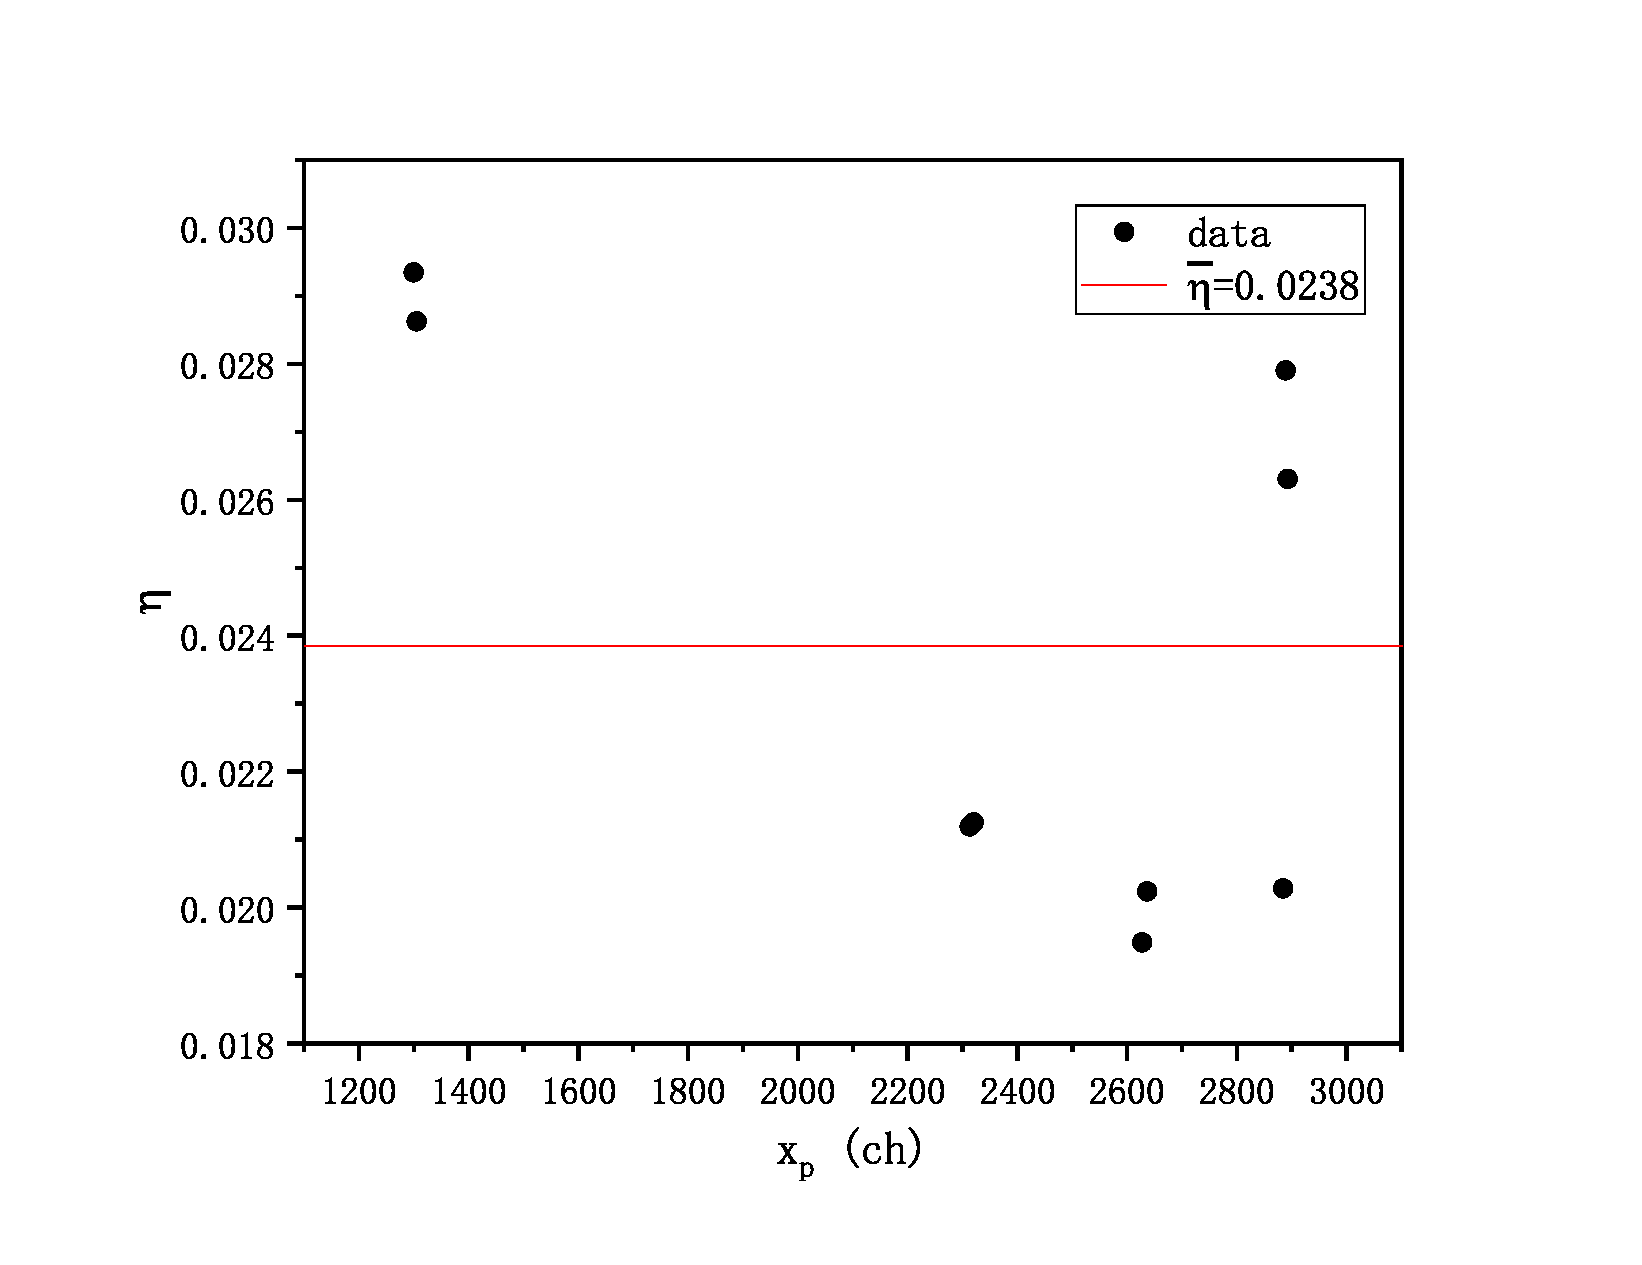
\includegraphics[width=1.1\linewidth]{eta.eps}
		\caption{$\eta-x_{\rm p} $图}
	\end{minipage}
	 \
	\begin{minipage}[t]{0.5\textwidth}
		\centering
		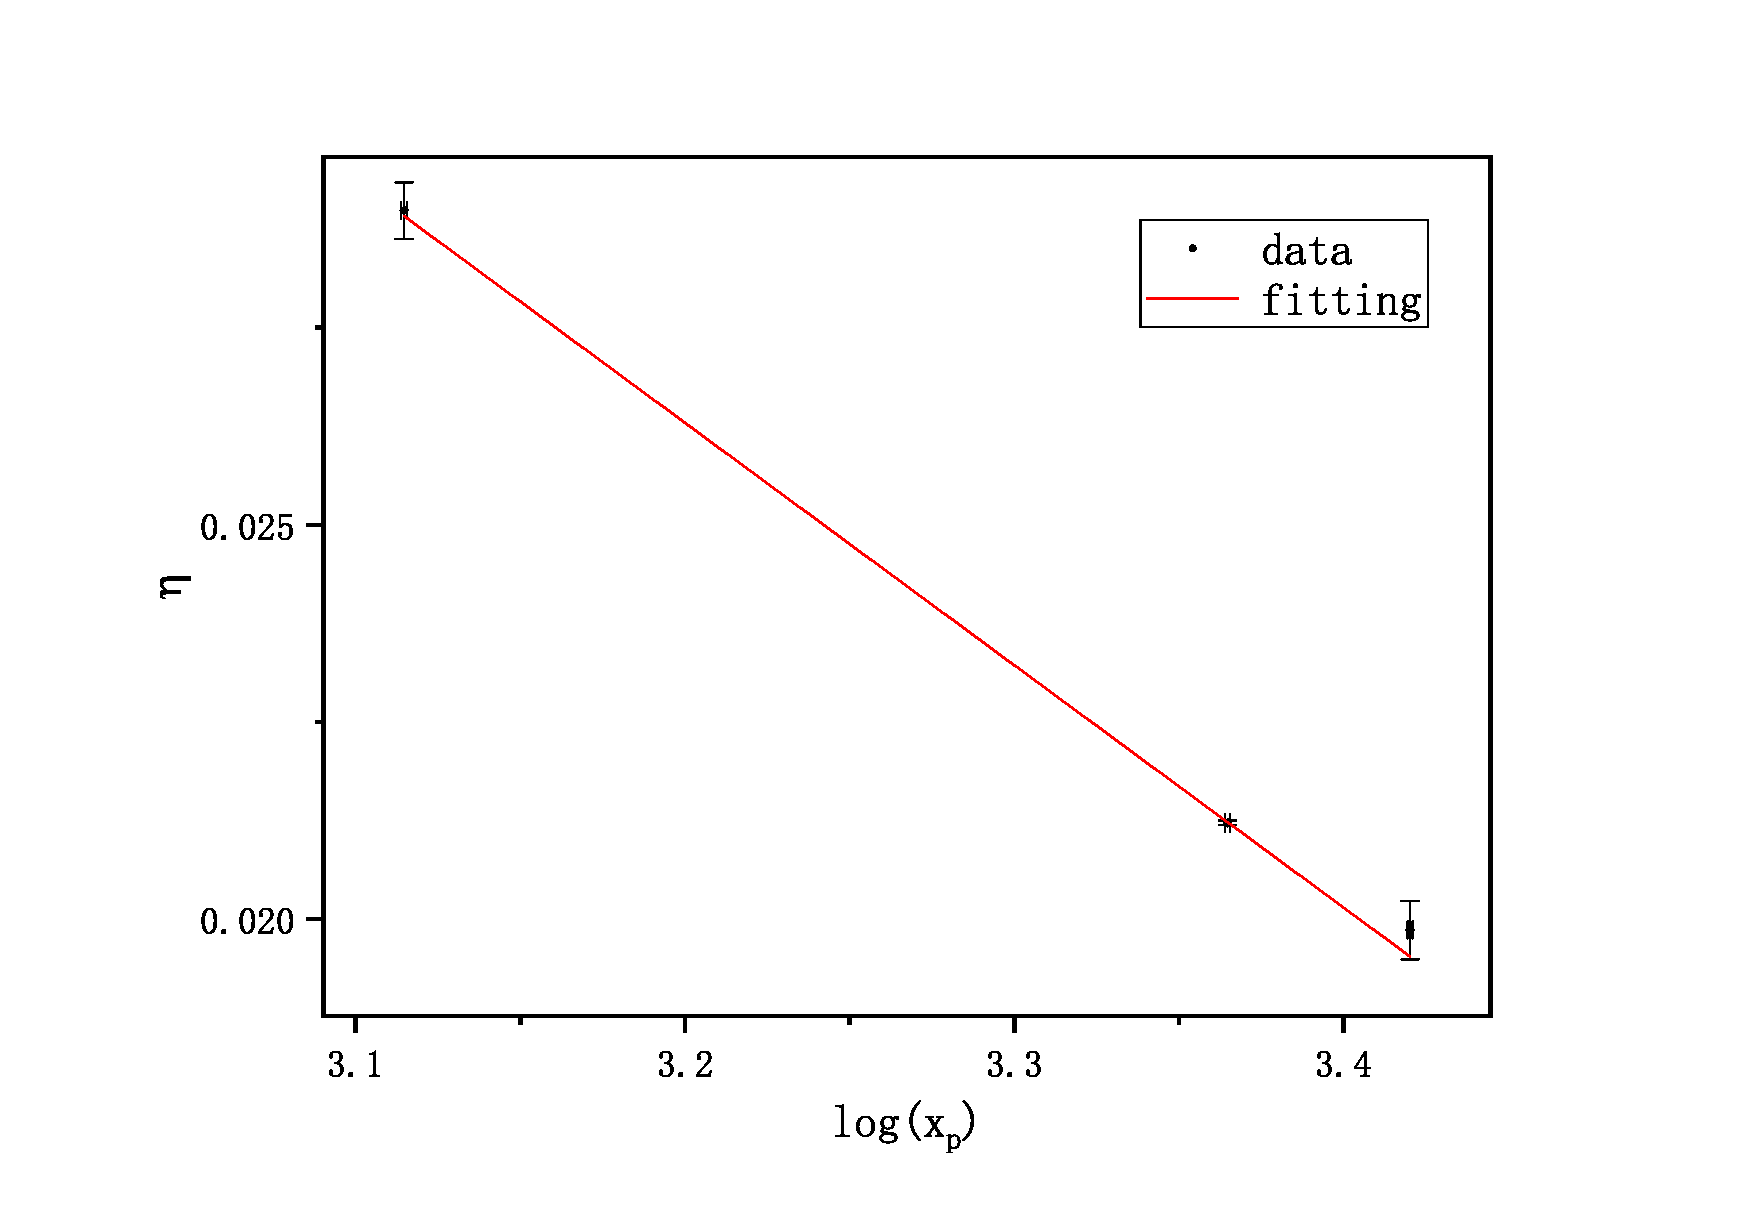
\includegraphics[width=1.1\linewidth]{eta-xp.eps}
		\caption{$ \eta-\log x_{\rm p} $曲线}
	\end{minipage}
\end{figure}
\subsection{$\rm ^{60}Co $贴近时的合成峰}
当$\rm ^{60}Co $贴近探测器时，理论上可以得到3个$ \gamma $峰，有一个峰为探测器同时吸收了$\rm ^{60}Co $的两个能量的$ \gamma $射线，实验中得到的峰如图8所示，对三个峰进行高斯拟合可得峰位(道址)：
\begin{equation*}
x_{\rm p1}=875.43\pm0.05,x_{\rm p2}=998.48\pm0.02,x_{\rm p3}=1902.37\pm0.06
\end{equation*}
\begin{figure}[H]
	\centering
	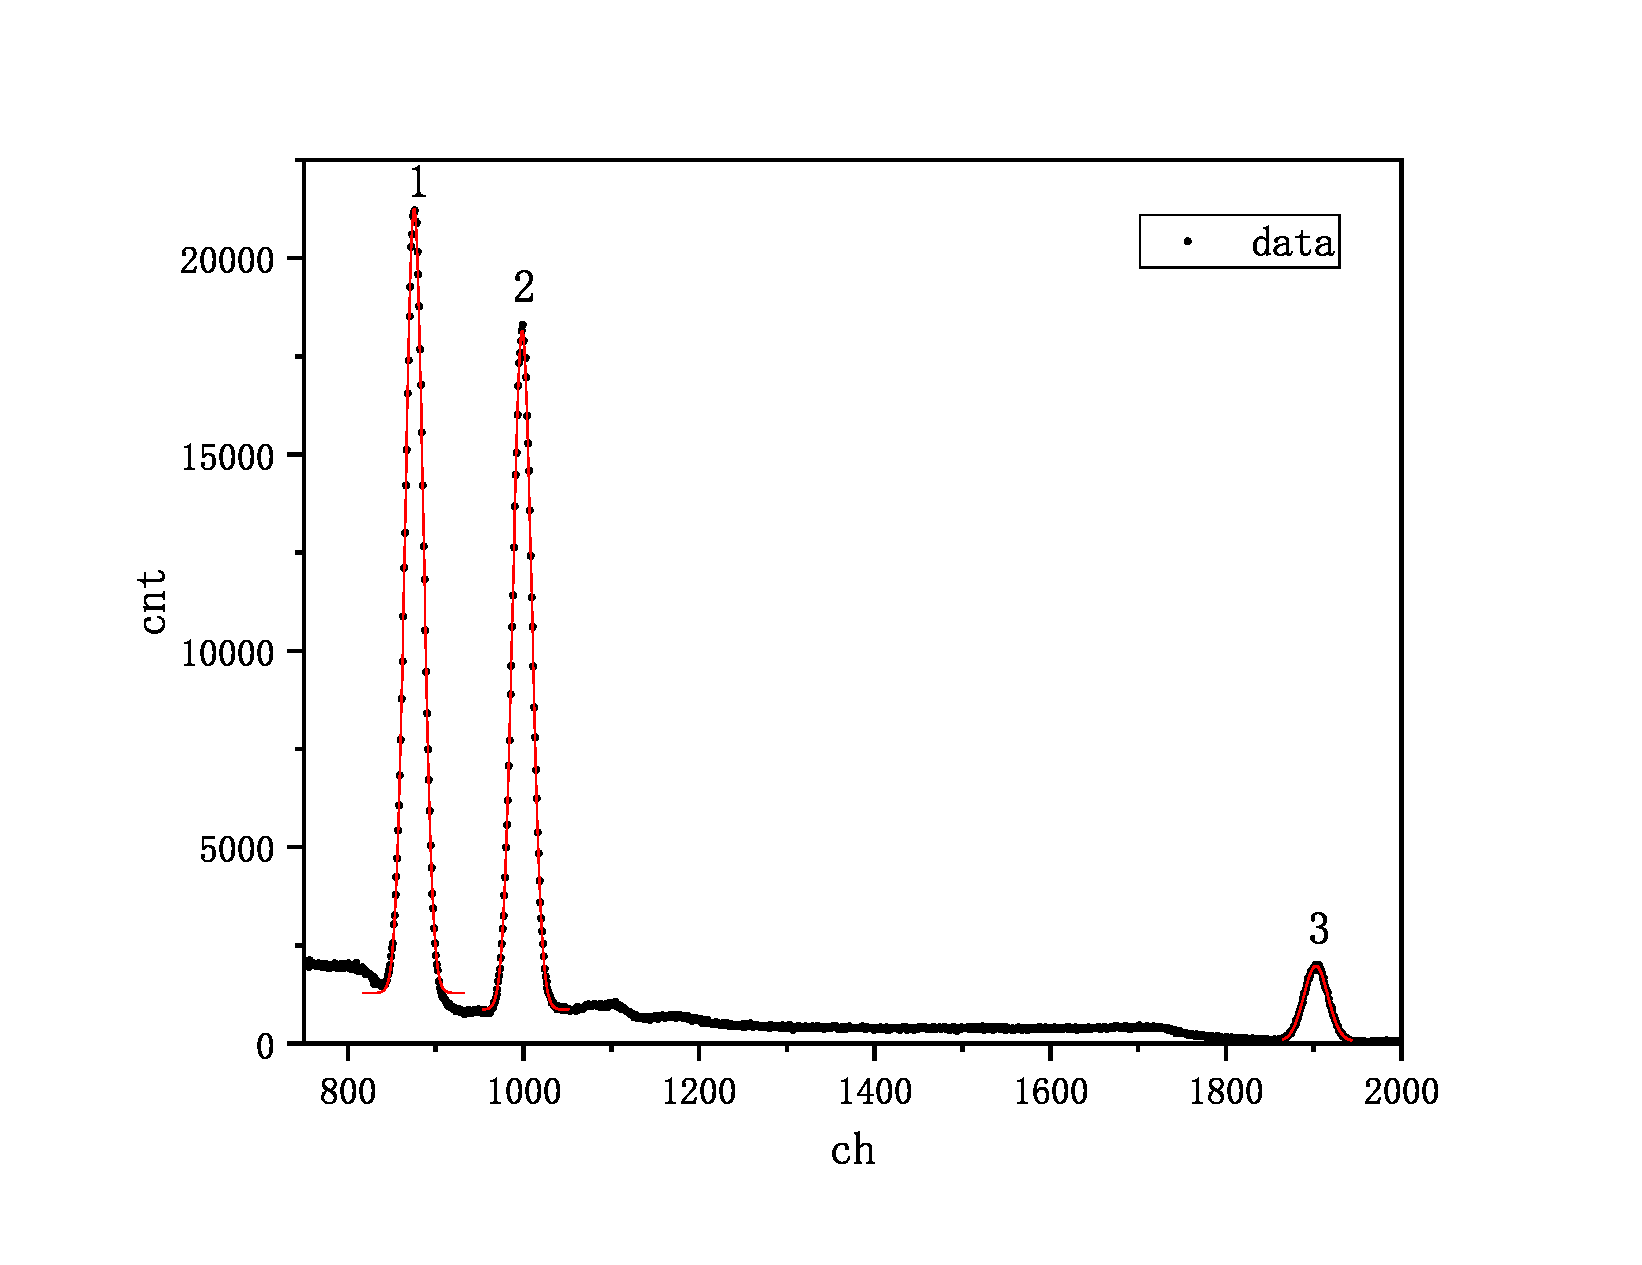
\includegraphics[width=0.9\linewidth]{Co60(close).eps}
	\caption{$\rm ^{60}Co $贴近时的$ \gamma $峰图}
\end{figure}
由于改变了放大器的放大倍数，用{$\rm ^{60}Co $的已知能量的两个$ \gamma $峰峰位对探测器重新进行能量刻度可得：
\begin{equation}
E(x_{\mathrm{p}})=(1.336\pm0.005)x_{\rm p}\pm4(\rm keV)
\end{equation}
把合成峰的峰位(道址)代入能量刻度函数可得：$ E(x_{\rm p_{3}})=(2542\pm10)\rm keV $。它与理论值2505keV接近，因而在实验误差允许的范围内，验证了合成峰的存在。

\subsection{环境本底相应的伽玛峰}
计数符合高斯分布，采用如下的函数族拟合：
\begin{equation}
y=y_{0}+\frac{A}{w \sqrt{\pi / 2}} e^{-2 \frac{\left(x-x_{\mathrm{c}}\right)^{2}}{w^{2}}}
\end{equation}
进行高斯拟合得到两个峰：
\begin{equation*}
x_{\rm c_{1}}=2859.53\pm3.09,\chi^{2}=33.453,R^{2}=0.964
\end{equation*}
\begin{equation*}
x_{\rm c_{2}}=2898.02\pm0.47,\chi^{2}=74.079,R^{2}=0.972
\end{equation*}
由此可得环境本底对应$ \gamma $射线的峰位(道址)为
\begin{equation}
x_{p_{1}}=x_{c_{1}}=2859.5\pm3.1
\end{equation}
\begin{equation}
x_{p_{2}}=x_{c_{2}}=2898.0\pm0.5
\end{equation}
相应的$ E_{\gamma_{1}}=(1451\pm5)\rm keV $，通过查阅相关资料得知它是放射源$\rm ^{40}K $衰变放出的$ \gamma $射线，$ E_{\gamma_{2}}=(1470\pm4)\rm keV $，通过查阅相关资料得知它是放射源$\rm ^{138}La $衰变放出的$ \gamma $射线，拟合效果如图9：
\begin{figure}[H]
	\centering
	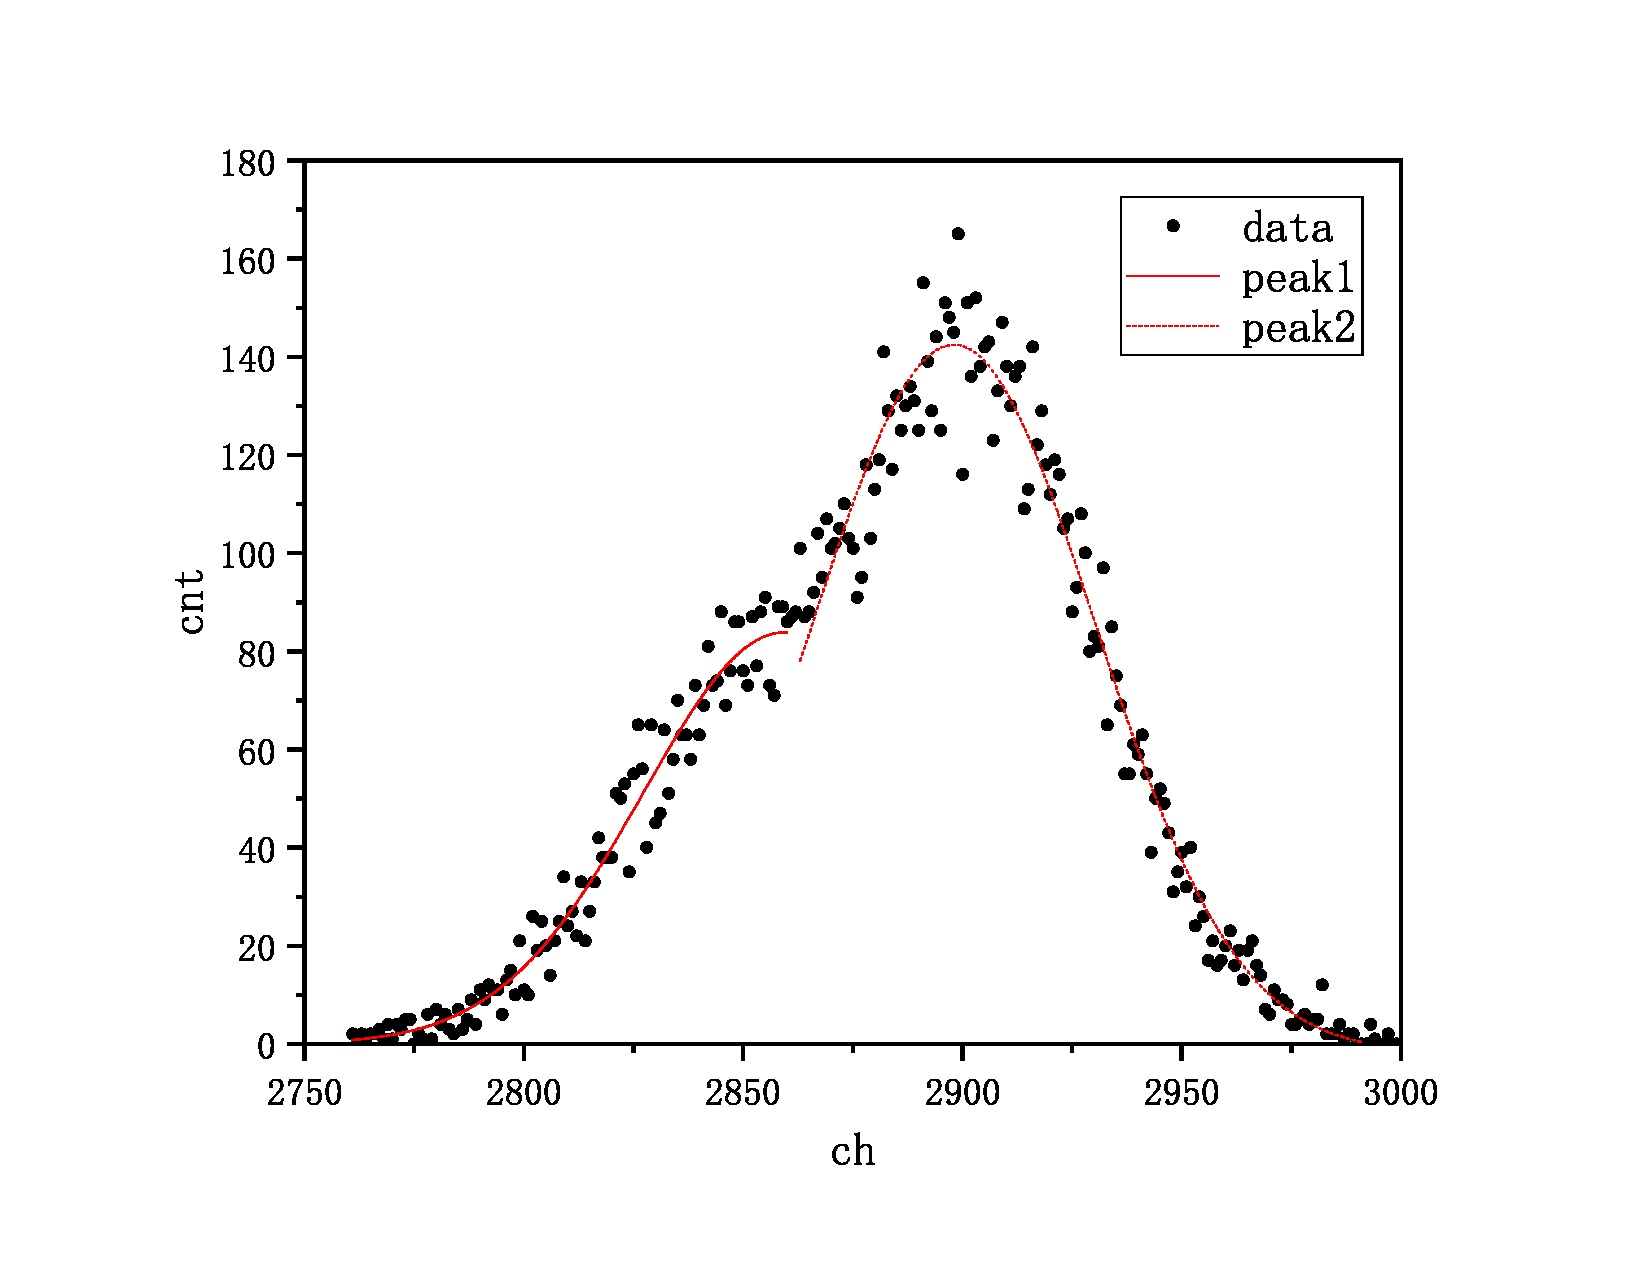
\includegraphics[width=0.9\linewidth]{background.eps}
	\caption{环境本底的$ \gamma $峰曲线}
\end{figure}

\section{误差分析}
\subsection{$\rm ^{60}Co $第一个峰的能量测定}
$\rm ^{60}Co $第一个峰的能量理论值是1173keV，测定值为$\rm (1173\pm3)keV $，相对误差为$ (0.0\pm0.2)\% $。误差来源主要为统计误差。
\subsection{$\rm ^{60}Co $贴近时的合成峰测定}
$\rm ^{60}Co $合成峰的能量理论值是2505keV，测定值为$\rm (2542\pm10)keV $，相对误差为$ (1.5\pm0.4)\% $。误差来源主要为探测时间不够长带来的统计误差。
\subsection{环境本底的$ \gamma $峰}
查阅相关资料可知，理论上，$\rm ^{40}K $源衰变放出的$ \gamma $射线能量为1461keV，测定值为$\rm (1451\pm5)ke $\\V，相对误差为$ (0.68\pm0.34)\% $，$\rm ^{138}La $源衰变放出的$ \gamma $射线和特征X射线符合相加效应得到的峰的能量为1468keV，测定值为$\rm (1470\pm4)keV $相对误差为$ (0.14\pm0.28)\% $。误差来源主要为两个峰相互重叠的影响，探测器的能量分辨率不足以使两个能量很相近的峰完全分离，以及测量时间不够长带来的统计误差。

\section{思考题}
\paragraph{1.实验中利用$\rm ^{60} Co $和$\rm ^{137} Cs $进行初步探测器标定，环境中的本底是否会影响，改变什么条件会使测量结果更加精确？}
会影响，可以放置铅块屏蔽本底，使结果更精确。

\paragraph{2.实验过程中测得$\rm ^{60} Co $和$\rm ^{137} Cs $ 能谱为什么会呈现连续分布？对于$\rm ^{60}Co$来说，1.17和1.33MeV的伽玛射线为级联跃迁，因此两者的计数应该是相同的，为什么在实验能谱上1.33MeV的伽玛峰计数会明显低于1.17MeV？}
(1)康普顿散射的连续谱从0到$ E_{\gamma}/(1+1/(4E_{\gamma})) $，全能峰有一定的展宽，环境本底的影响。
(2)能量越高，探测器的探测效率越低。

\paragraph{3.高于1.3MeV会出现一些本底峰？如何更准确的进行定标。}
会，增加测量时间使峰变得明显。

\section{实验总结}
本次实验使用NaI(TI)探测器进行$ \gamma $射线能谱的测定，并进行了能量刻度，探究了能量分辨率与射线能量的关系，还进行了本底放射源的分析，收获颇多。了解了$ \gamma $射线与物质相互作用的基本原理，学会了该闪烁体探测器的使用，掌握了相关的数据处理和分析方法，并且在数据处理和撰写实验报告中熟悉了对Origin和\LaTeX{}的使用，实验和数据处理能力大大提高。另外，之前老师理论课上讲的通过实践获得了更深的理解，掌握更牢。

\end{document}